\chapter{Experiments and results}

This chapter describes the experiments we performed to show the effectiveness of the proposed method. 

\section{Evaluation datasets}
To quantitatively evaluate the proposed methods, and to compare it to related work,
we considered two datasets: the DSO-1 and DSI-1 datasets\footnote{Public available for download at https://recodbr.wordpress.com/code-n-data}. Each dataset comes with a face position groundtruth and a splicing region mask. Additionally, the ColorChecker dataset \cite{gehler2008bayesian} is used as a source of pristine images.

The latter dataset has been mainly used for experimenting on pristine data: due to its characteristics it is very varied and lends itself well to image analysis based on color.

\subsection{DSO-1}

The DSO-1 dataset is composed of 200 indoor and outdoor images with the resolution of 2048 × 1536 pixels. Out of this set of images, 100 are original, i. e. they have no adjustments, and 100 are forged. 

\begin{figure}[!htb]
\minipage{0.48\textwidth}
  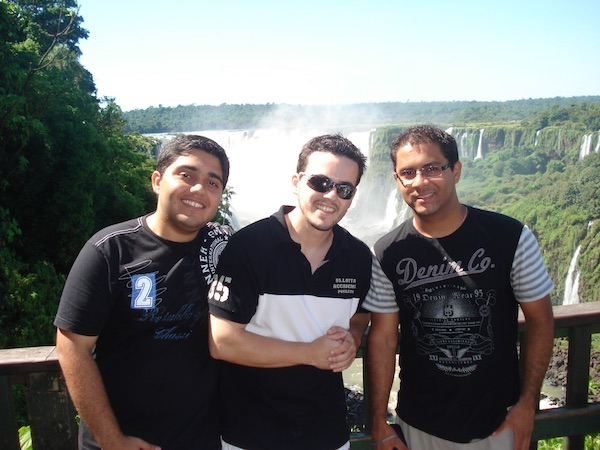
\includegraphics[width=\linewidth]{dso_sample}
  \caption{DSO-1 sample original image}\label{fig:dsooriginalimage}
\endminipage\hfill
\minipage{0.48\textwidth}
  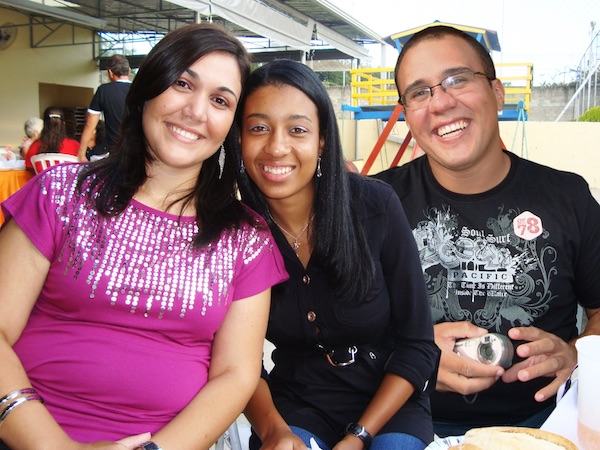
\includegraphics[width=\linewidth]{dso_sample_spliced}
  \caption{DSO-1 sample spliced image}\label{fig:dsosplicedimage}
\endminipage
\end{figure}

The forgeries were created by adding one or more individuals in a source image that already contained one or more people. When necessary, some post-processing operations were made (such as color and brightness adjustments) in order to increase photorealism.

\subsection{DSI-1}

The DSI-1 dataset is composed of 50 images with different resolutions (25 original and 25 doctored) downloaded from different websites in the Internet. Original images were downloaded from Flickr and doctored images were collected from different websites such as \emph{Worth 1000}, \emph{Benetton Group 2011}, \emph{Planet Hiltron}, etc.

\begin{figure}[!htb]
\minipage{0.46\textwidth}
  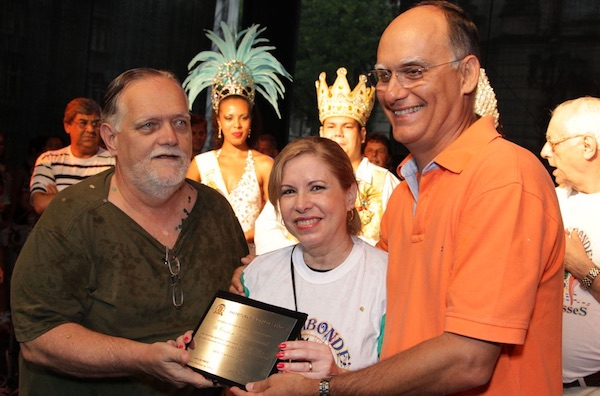
\includegraphics[width=\linewidth]{dsi_sample_normal}
  \caption{DSI-1 sample original image}\label{fig:dsioriginalimage}
\endminipage\hfill
\minipage{0.50\textwidth}
  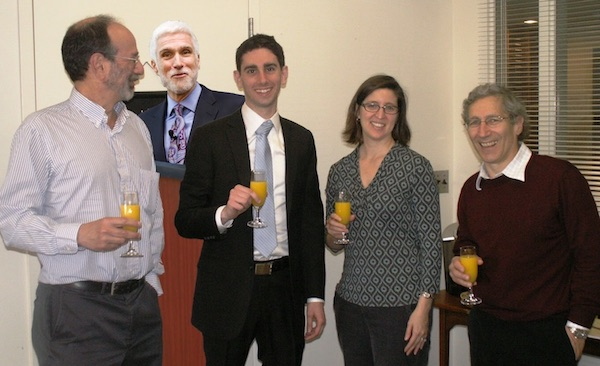
\includegraphics[width=\linewidth]{dsi_sample_spliced}
  \caption{DSI-1 sample spliced image}\label{fig:dsisplicedimage}
\endminipage
\end{figure}

\subsection{ColorChecker}

The ColorChecker dataset is a collection of images for evaluating Color Constancy algorithms built as additional material to \cite{gehler2008bayesian}. It consists in 568 RGB colored images of different scenes, both indoor and outdoor taken under different illuminations. In each scene a \emph{Gretag MacBeth Color Checker Chart}\footnote{The \emph{ColorChecker} consists in a rectangular card measuring about 11 × 8.25 inches containing a series of six gray patches, plus typical additive (Red-Green-Blue) and subtractive (Cyan-Magenta-Yellow) primaries, plus other \emph{natural} colors such as light and dark skin, sky-blue, foliage, etc. It is usually used for color calibration of digital cameras. The color pigments were selected for optimum color constancy when comparing pictures of the chart with pictures of the natural colors. The ColorChecker was introduced in a 1976 paper by McCamy, Marcus, and Davidson in the \emph{Journal of Applied Photographic Engineering} \cite{mccamy1976color}.}  was placed such that it was illuminated by the main scene illuminant and thus its color could be retrieved. The data is available in Canon RAW format free of any correction.

\begin{figure}[h!]
  \centering
    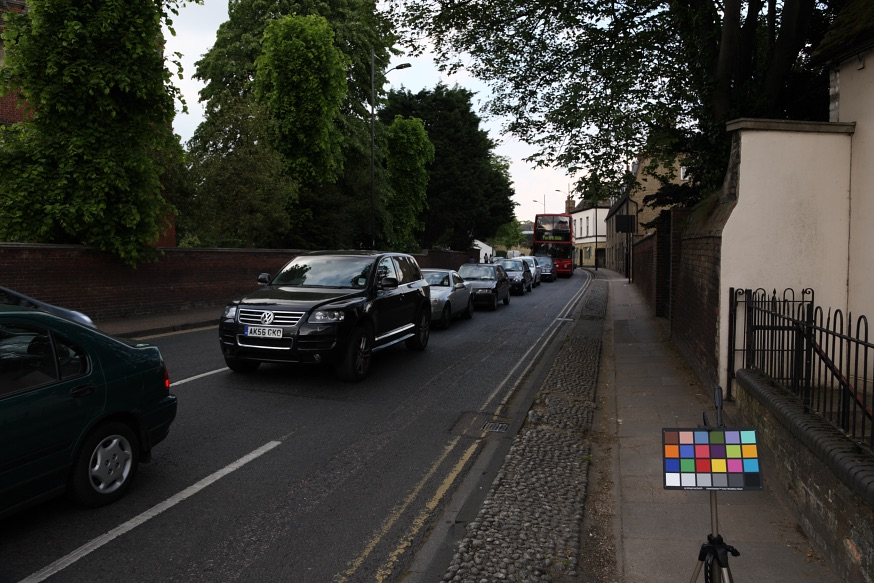
\includegraphics[width=0.65\textwidth]{colorchecker_sample}
    \caption{Example of an image of the ColorChecker dataset}
    \label{fig:colorcheckersample}
\end{figure}

\section{Face forgery detection module performance}

This section describes the experiments performed to evaluate the face forgery detection module. In these experiments, the DSO-1 and the DSI-1 datasets are used for evaluation.

After having characterized an image with a specific image descriptor, the next step consists of training a classifier (a kNN model in our case).

The proposed method focuses on using complementary information (i.e the color descriptors) to describe the computed \emph{illuminant maps}. Accordingly to Carvalho \emph{et al. }\cite{carvalho2016illuminant}, we selected the \emph{k-Nearest Neighbor (kNN)} classifier instead of more powerful and computational intensive ones such as \emph{Support Vector Machines (SVM)} due to the fact that the two types of classifiers (or even fusion of both learning methods) present very similar results. For that reasons, a simpler learning techinque is chosen\cite{carvalho2016illuminant}. As in \cite{carvalho2016illuminant}, the value of \emph{k} for the kNN classifiers is set to 5. 

For all considered color descriptors (ACC, BIC, CCV and LCH), we have used the standard configuration proposed by Penatti \emph{et al.} \cite{penatti2012comparative}. As described in Chapter 2, eight different kNN models are trained and used for the classification, considering all the possible combinations of the couples composed by a IMs transformed space (GGE e IIC)and a color descriptor (chosen from ACC, BIC, CCV and LCH).

\subsection{Color descriptors accuracies}

Since the final classification output is given by majority voting of all the selected classifiers, the first round of experiments aimed at evaluating the accuracy of each image descriptors.

\begin{table}[h!]
\centering
\begin{tabular}{l c c c c c c} 
\hline \hline 
\textbf{Test case} & \textbf{Train} & \textbf{Test} & \textbf{ACC} & \textbf{BIC} & \textbf{CCV} & \textbf{LCH} \\ [0.5ex]
\hline
Test 1 & DSO-1 & DSO-1 &	0.75 & 0.75	& 0.72 & \textbf{0.78}\\
Test 2 & DSI-1 & DSI-1 &	0.78 & 0.79 & 0.77 & \textbf{0.82}\\
Test 3 &	DSO-1 &	DSI-1 &	0.56 & \textbf{0.57} & 0.53 & 0.53\\
Test 4 &	DSI-1 & DSO-1 & 0.58 & 0.55 & 0.51 & \textbf{0.59}\\ [1ex]
\hline
\end{tabular}
\caption{Accuracy for kNN technique using a single color descriptor. Experiments are performed using 10-fold cross-validation in test case number 1 and 2.}
\label{table:colordescriptorperformance}
\end{table}

Table \ref{table:colordescriptorperformance} shows the results of all tested combinations of training and test set. The classification results show that, generally, LCH color descriptor yielded the higher accurary, but there is not a descriptor that outperforms the others.

\subsection{Test cases}

After analyzing each single descriptor accuracy, we proceeded to evaluate the overall module performance using a combination of all of them, as described in Chapter 2. Since not all the color descriptors perform equally, a different weight $w$ is given at each classifier. Thus, the Eq.(\ref{eq:faceknnscores}) presented in Chapter 2 becomes:

\begin{equation}
Score(\mathcal{P}) = \sum_{i = 1}^{8} w_i * prediction_{C_i}(\mathcal{P})
\end{equation}

where $\mathcal{P}$ is the considered paired face feature, $C_i$ is the $i$-th kNN classifier, $prediction_{C_i}(\mathcal{P}) \in [0, 1]$ and $w_i \geq 1 \; \forall i = 1, \ldots, 8$.

In the following experiments, the  method has been applied for classifying a face pair as fake or real using uniform (Table \ref{table:performancefacedet}) and non-uniform (Table \ref{table:performancefacedetnonun}) weights. Essentially, these experiments evaluate the forgery detection performances of the face detector module.

For each test case in the suite it is reported:
\begin{enumerate}
\item The training dataset (\textbf{\emph{Train}});
\item The evaluation dataset (\textbf{\emph{Test}});
\item The classification accuracy score (\textbf{\emph{ACC}});
\item The area under the \emph{Receiver Operator Characteristic (ROC)} curve (\textbf{\emph{AUC}})
\item The accuracy score expressed through the $F_1$ score (also known as \textbf{\emph{F-Score}})
\end{enumerate}

Accordingly with Jeni \emph{et al.} \cite{jeni2013facing}, when dealing with AUC score to measure the performance of classifier, one of the major drawbacks relies on the fact that an increasing of AUC doesn't really mean a better classifier, but it could be just the side-effect of too many negative examples used in training.

Therefore, another classification accuracy score is also provided, the \emph{F-Score}. 

Let the classification \emph{precision} score given by

$$
precision = \frac{TP}{TP + FP}
$$

where $TP$ and $FP$ are true positives and false positives respectively.

The classification \emph{recall} value is defined as
$$
recall = \frac{TP}{TP + FN}
$$
where $FN$ stands for false negatives. The $F_{\beta}$ score is defined as the harmonic mean of \emph{precision} and \emph{recall} values:

\begin{equation}
F_{\beta} = (1 + \beta^2) * \frac{precision * recall}{(\beta^2 * precision) + recall}
\end{equation}

where $\beta$ states for the relative importance given to precision comparing to recall. In our experiments, we considered $\beta = 1$ (\emph{i.e.} the $F_1$ score), so:
\begin{equation}
F_{1} = 2 * \frac{precision * recall}{precision + recall}  = \cdots = \frac{2 * TP}{2 * TP + FP + FN}
\end{equation}

In order to proceed with the comparison between using uniform and non-uniform weights for classifiers, we had to determine the most appropriate weight values for each descriptor. These values have been found with an exhaustive search by evaluating the performance of the currently analyzed weights combination over the DSO-1 dataset with a 10-fold cross-validation protocol. 

To reduce the computational cost, we limited the range of values to be explored for each classifier basing on the results reached for each single descriptor (presented in Table \ref{table:colordescriptorperformance}) giving more importance to LCH descriptor. Table \ref{table:classifiersweights} reports the used classifiers weights.

\begin{table}[h!]
\centering
\begin{tabular}{l c} 
\hline \hline 
\textbf{Descriptor} & \textbf{Weight}\\ [0.5ex]
\hline
ACC & 1.10\\
BIC & 1.25\\
CCV & 1\\
LCH & 1.56\\ [1ex]
\hline
\end{tabular}
\caption{The weights used for each classifier in the non-uniform case.}
\label{table:classifiersweights}
\end{table}

Experimental results are collected in Table \ref{table:performancefacedet}, for the uniform weights case, and in Table \ref{table:performancefacedetnonun}, for non-uniform case. 

\begin{table}[h!]
\centering
\begin{tabular}{l c c c c c} 
\hline \hline 
\textbf{Test case} & \textbf{Train} & \textbf{Test} & \textbf{ACC} & \textbf{AUC} &\textbf{ F-Score} \\ [0.5ex]
\hline
Test 1 & DSO-1 & DSO-1 &	0.82 & 0.88	& 0.77\\
Test 2 & DSI-1 & DSI-1 &	0.87 & 0.92 & 0.87\\
Test 3 &	DSO-1 &	DSI-1 &	0.58 & 0.58 & 0.62\\
Test 4 &	DSI-1 & DSO-1 & 0.62 & 0.59 & 0.53\\ [1ex]
\hline
\end{tabular}
\caption{Performance of face forgery detection module over paired faces using uniform weights.}
\label{table:performancefacedet}
\end{table}

\begin{table}[h!]
\centering
\begin{tabular}{l c c c c c} 
\hline \hline 
\textbf{Test case} & \textbf{Train} & \textbf{Test} & \textbf{ACC} & \textbf{AUC} &\textbf{ F-Score} \\ [0.5ex]
\hline
Test 1 & DSO-1 & DSO-1 &	0.84 & 0.90	& 0.78\\
Test 2 & DSI-1 & DSI-1 &	0.89 & 0.92 & 0.89\\
Test 3 &	DSO-1 &	DSI-1 &	0.59 & 0.58 & 0.64\\
Test 4 &	DSI-1 & DSO-1 & 0.63 & 0.60 & 0.54\\ [1ex]
\hline
\end{tabular}
\caption{Performance of face forgery detection module over paired faces using non-uniform weights.}
\label{table:performancefacedetnonun}
\end{table}

Resulting accuracy scores are obtained as average over 5 consecutive runs of the algorithm. For a better visualization, Figure \ref{fig:compareknnweights} depicts a direct comparison between the accuracy of both experimental results as a bar graph.

\begin{figure}[h!]
  \centering
    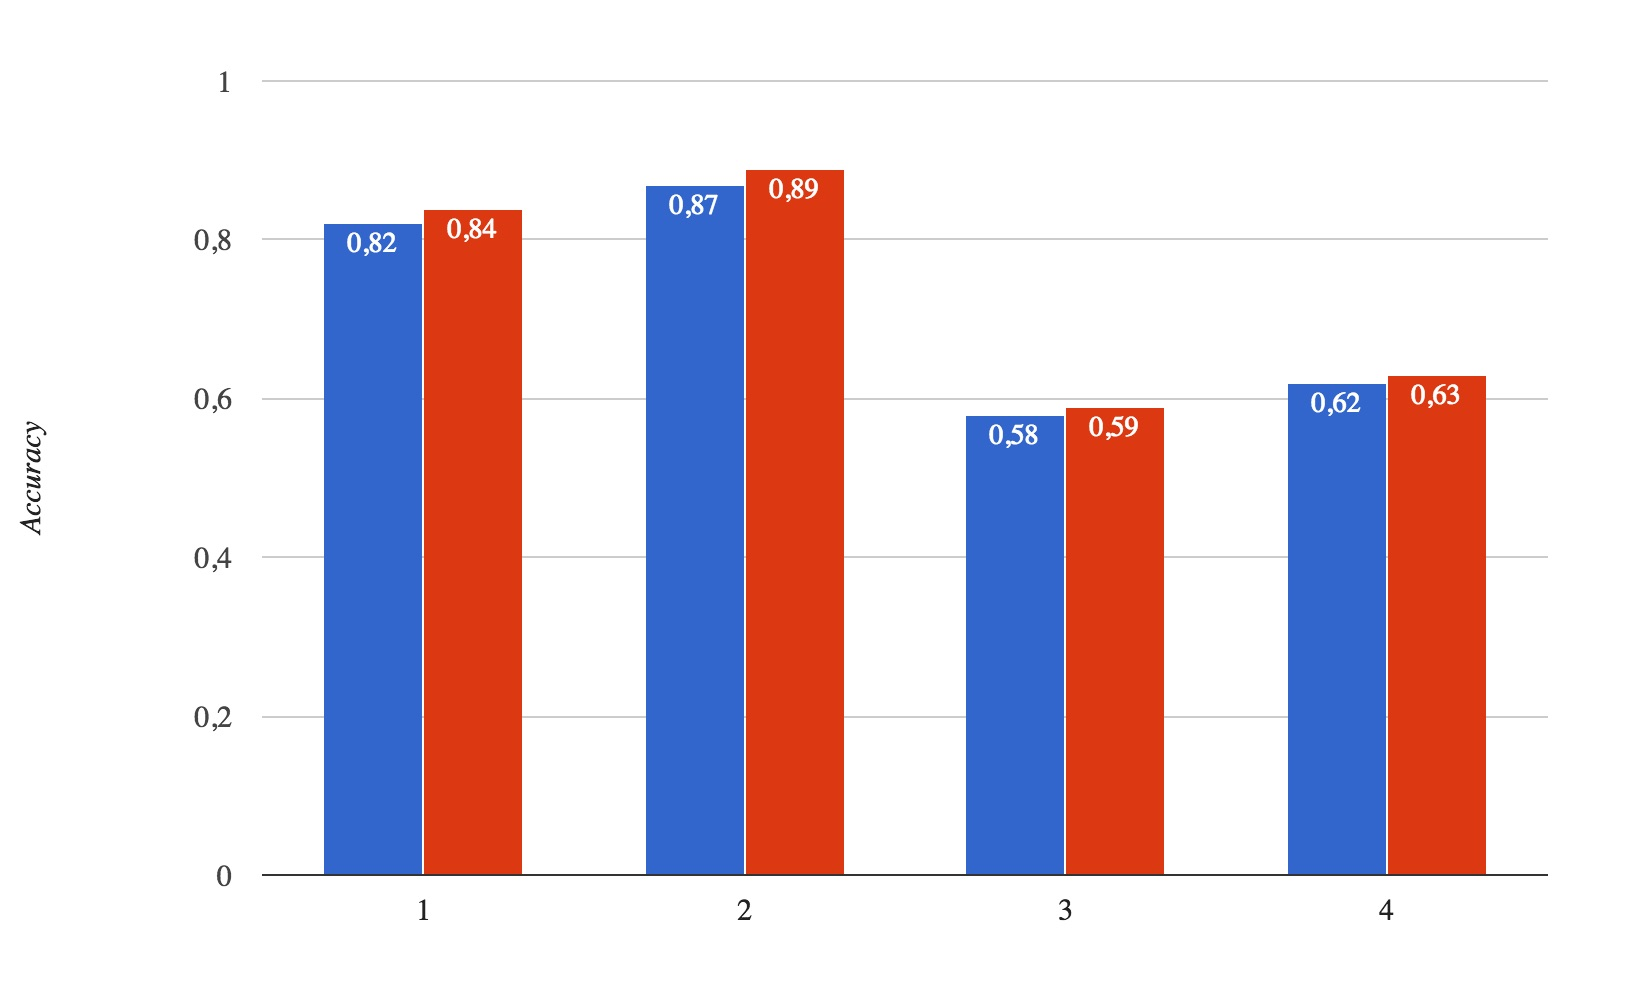
\includegraphics[width=0.9\textwidth]{compareknnweights}
    \caption{Classification accuracies comparison between using uniform and non uniform weights for kNN classifiers over the considered 4 test cases of Table \ref{table:performancefacedet}. The blue bins depict the reached accuracies using uniform weights, reds are for non-uniform case.}
    \label{fig:compareknnweights}
\end{figure}

These results show that, although we can notice a slight performance improvement in all test cases, the use of non-uniform weights do not affect much the final classification results.

In the following subsections are described the experimental results for each analyzed test case using non-uniform weights. We show results using classical \emph{Receiver Operator Characteristic (ROC)} \cite{fawcett2006introduction} and \emph{Precision-Recall} curves\cite{Davis:2006:RPR:1143844.1143874}. 

\subsubsection{Performance on DSO-1 dataset}

In this experiment, we applied the proposed method for classifying a face pair as fake or real considering only the DSO-1 dataset. We reached an average accuracy of 84\% using the 10-fold cross-validation protocol.

\begin{figure}[!htb]
\minipage{0.42\textwidth}
  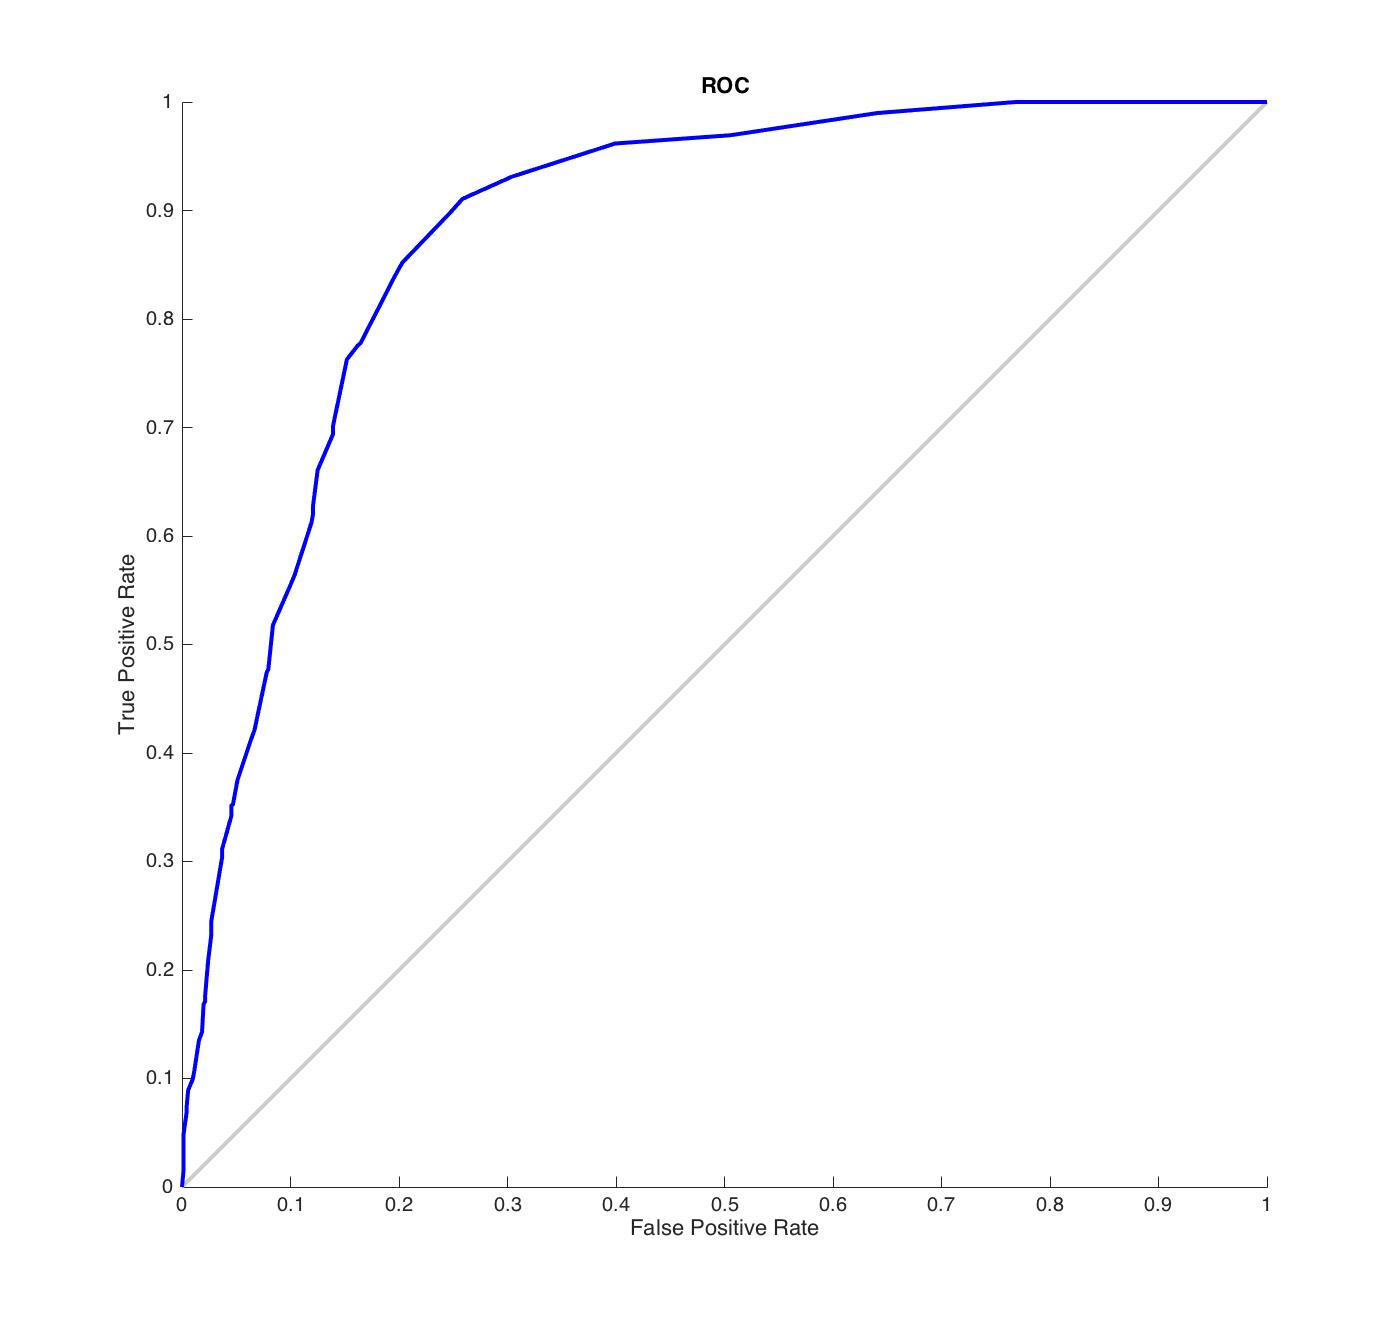
\includegraphics[width=\linewidth]{train_dso_crossvalidation}
\endminipage\hfill
\minipage{0.53\textwidth}
  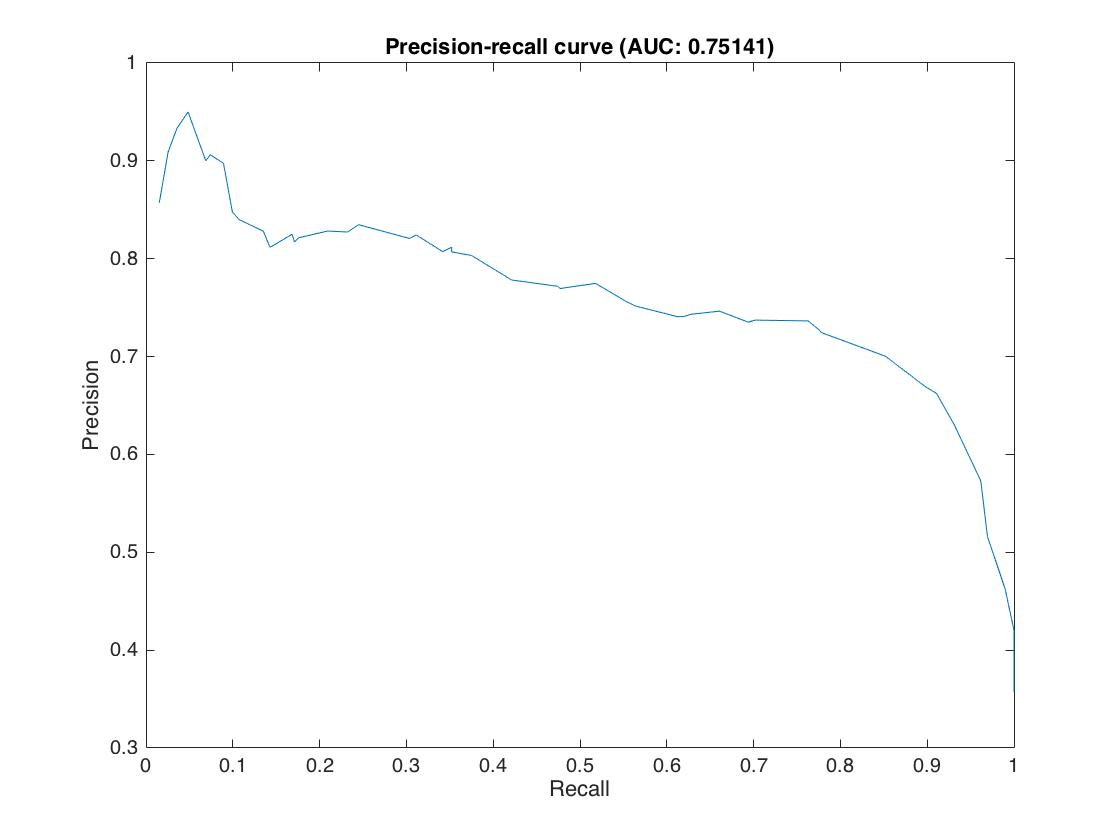
\includegraphics[width=\linewidth]{train_dso_crossvalidation_prec_rec}
\endminipage
\caption{ROC curve and Precision-Recall curve for DSO-1 cross-validation classification of paired faces.}\label{fig:regiondetnormal}
\end{figure}

\subsubsection{Performance on DSI-1 dataset}

In this experiment we applied the proposed method for classifying a face pair as fake or real considering only the DSI-1 dataset. We reached an average accuracy of 89\% using the 10-fold cross-validation protocol.

\begin{figure}[!htb]
\minipage{0.42\textwidth}
  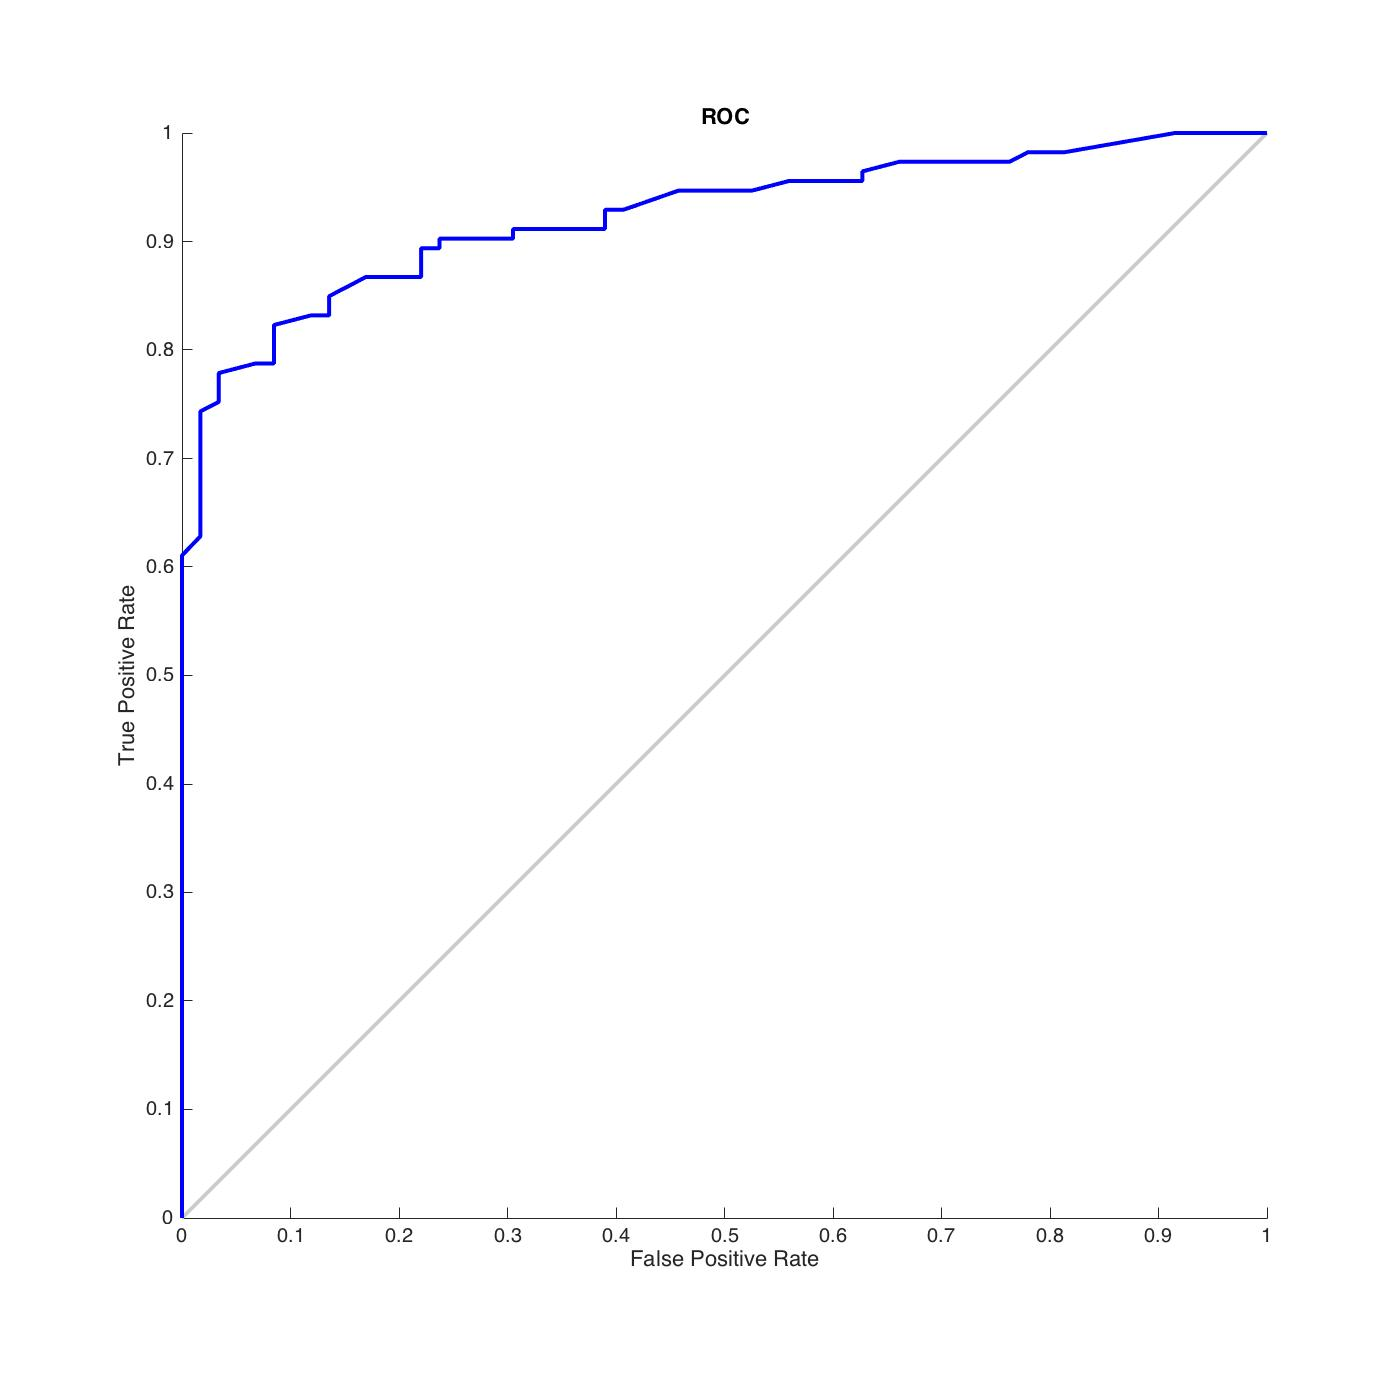
\includegraphics[width=\linewidth]{train_dsi_crossvalidation}
\endminipage\hfill
\minipage{0.53\textwidth}
  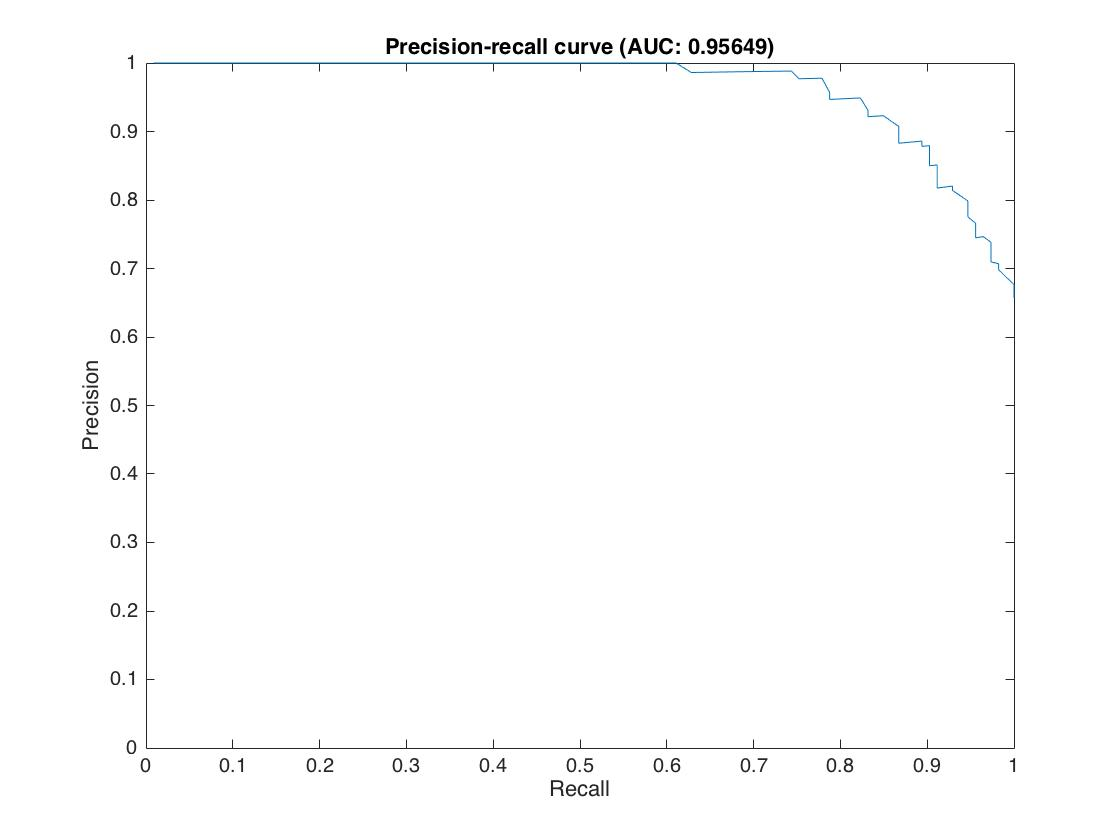
\includegraphics[width=\linewidth]{train_dsi_crossvalidation_prec_rec}
\endminipage
\caption{ROC curve and Precision-Recall curve for DSI-1 cross-validation classification of paired faces.}\label{fig:regiondetnormal}
\end{figure}

\subsubsection{Cross dataset performance on DSO-1}

In this experiment we performed a cross-dataset validation in which we trained our method with images from DSI-1 and test it against images from the DSO-1 dataset. We achieved an average classification accuracy of 63\%. 

\begin{figure}[!htb]
\minipage{0.42\textwidth}
  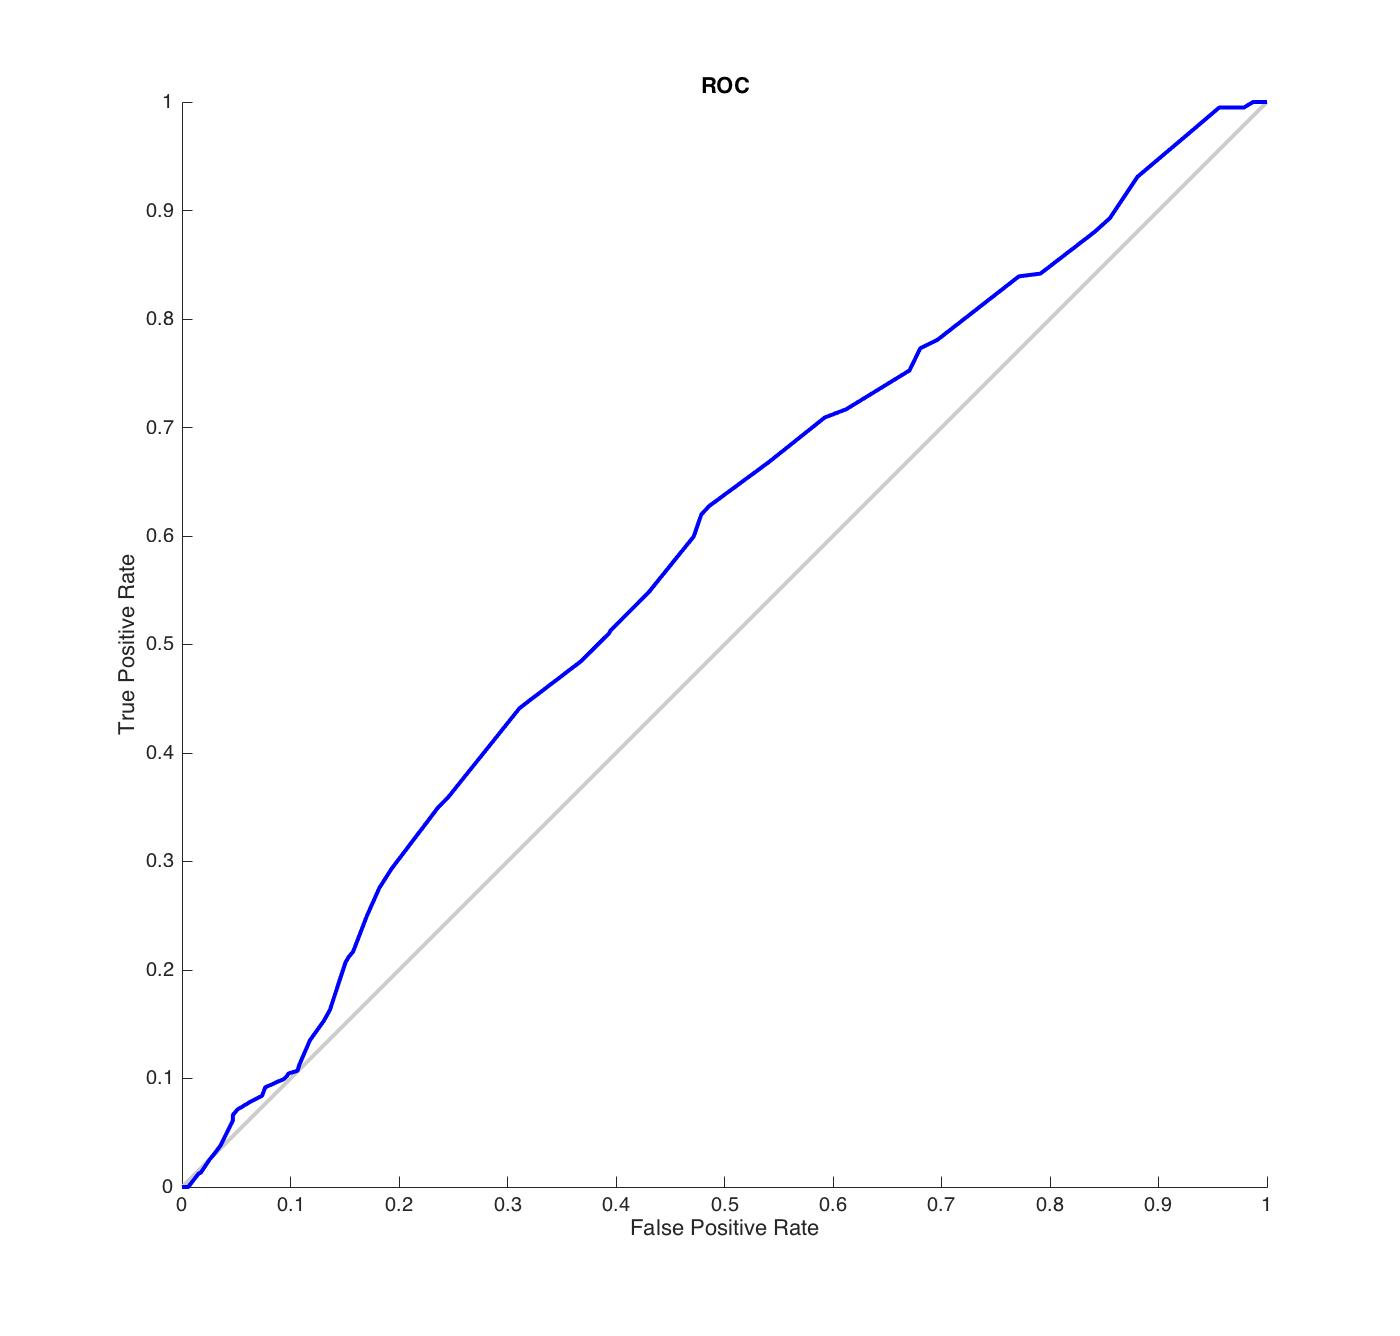
\includegraphics[width=\linewidth]{train_dsi_test_dso}
\endminipage\hfill
\minipage{0.53\textwidth}
  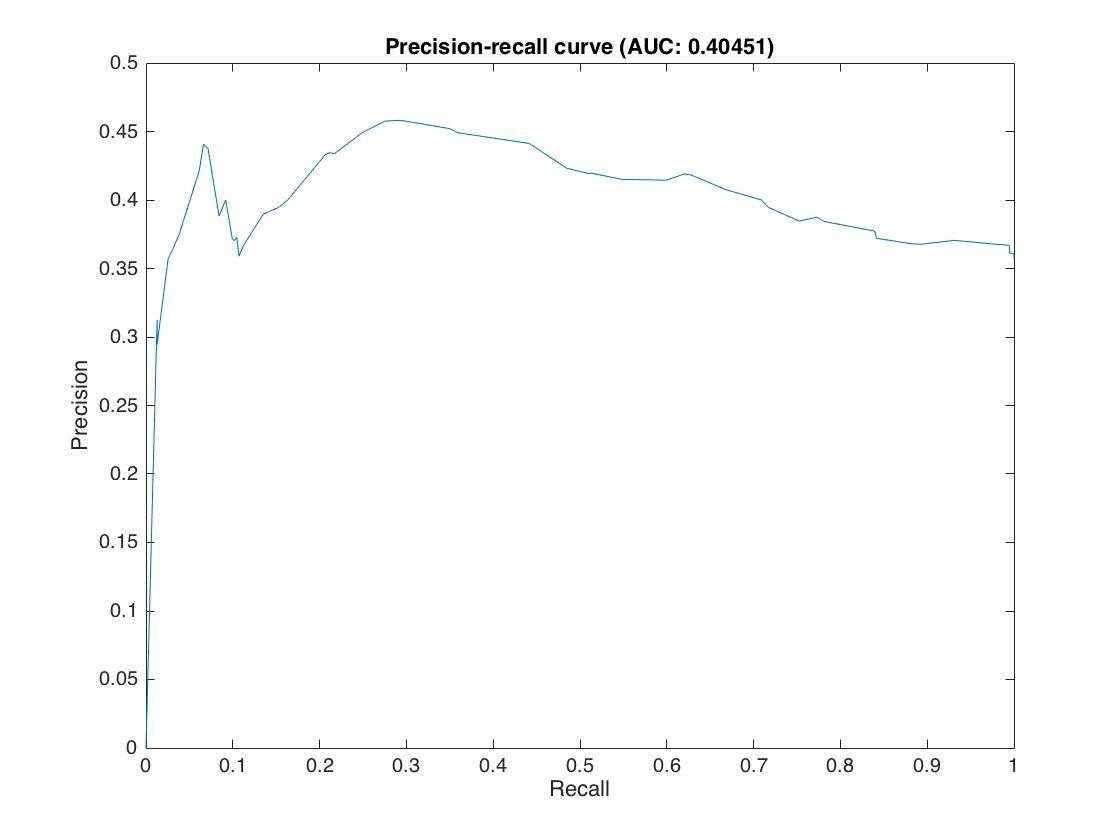
\includegraphics[width=\linewidth]{train_dsi_test_dso_prec_rec}
\endminipage
\caption{ROC curve and Precision-Recall curve for DSO-1 paired faces classification using trained data on DSI-1.}\label{fig:regiondetnormal}
\end{figure}

\subsubsection{Cross dataset performance on DSI-1}

In this experiment we performed a cross-dataset validation in which we trained our method with images from DSO-1 and test it against images from the Internet (DSI-1). We achieved an average classification accuracy of 59\%. 

\begin{figure}[!htb]
\minipage{0.42\textwidth}
  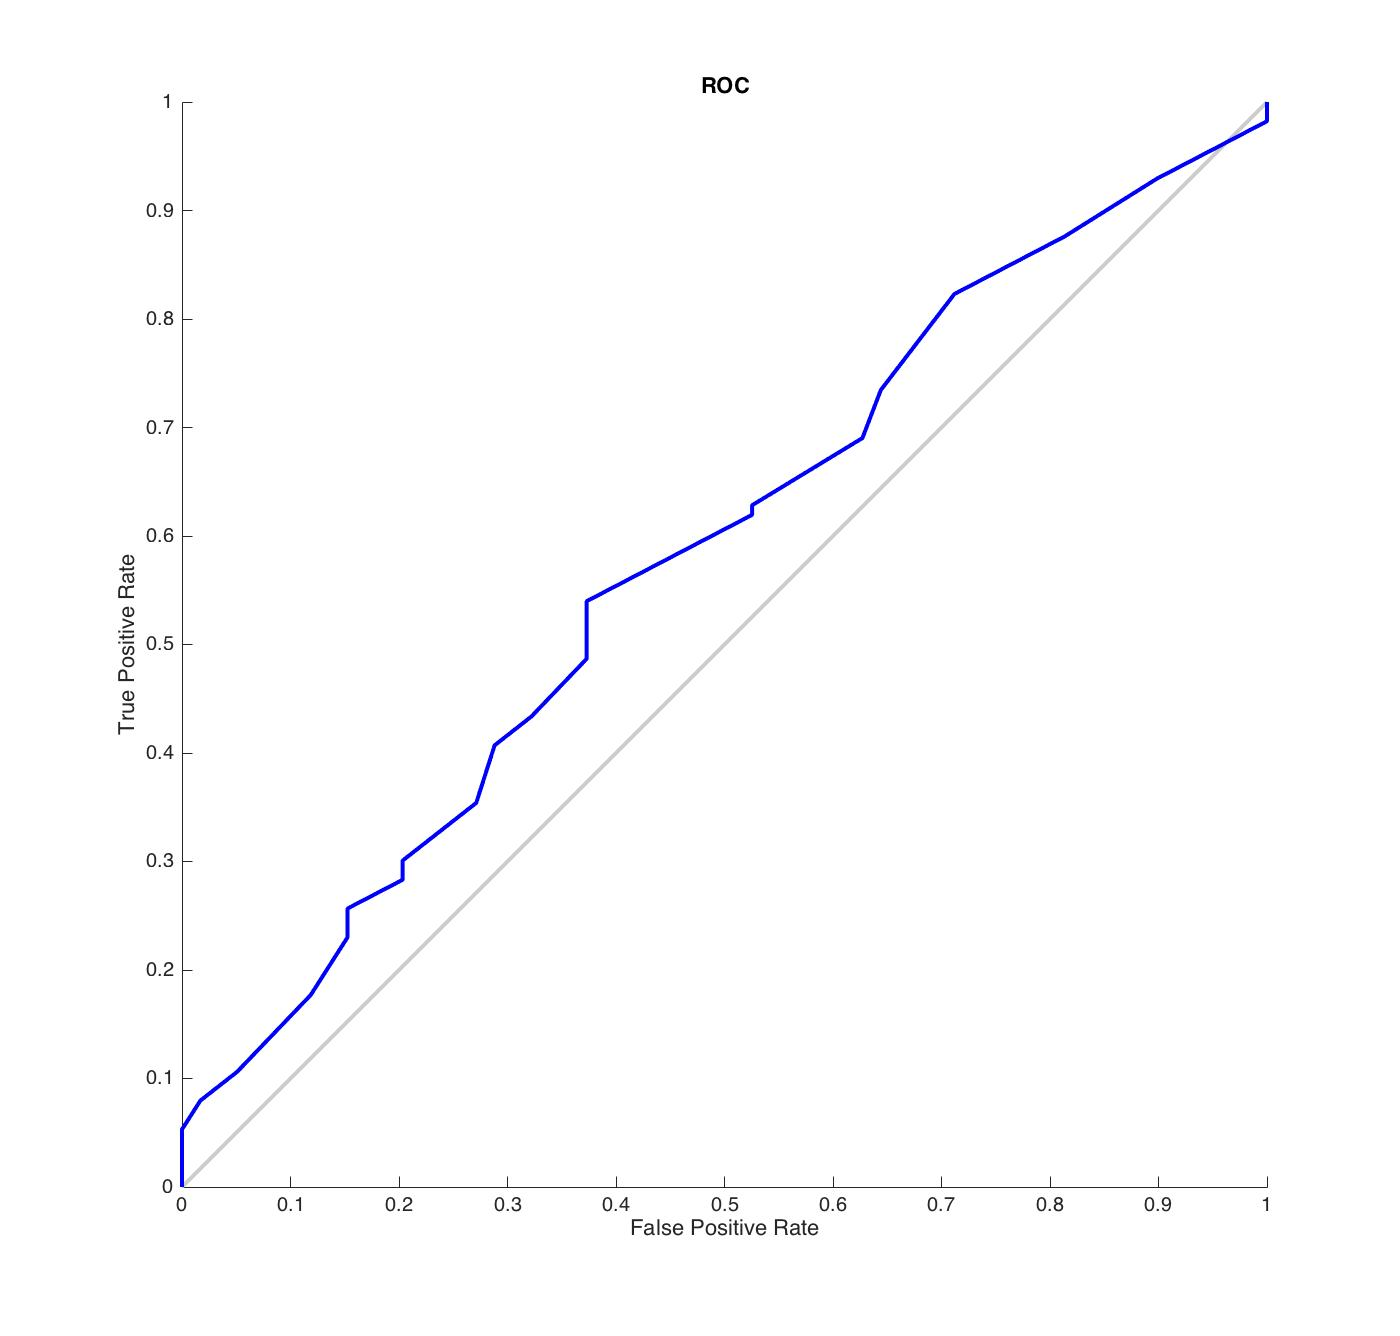
\includegraphics[width=\linewidth]{train_dso_test_dsi}
\endminipage\hfill
\minipage{0.53\textwidth}
  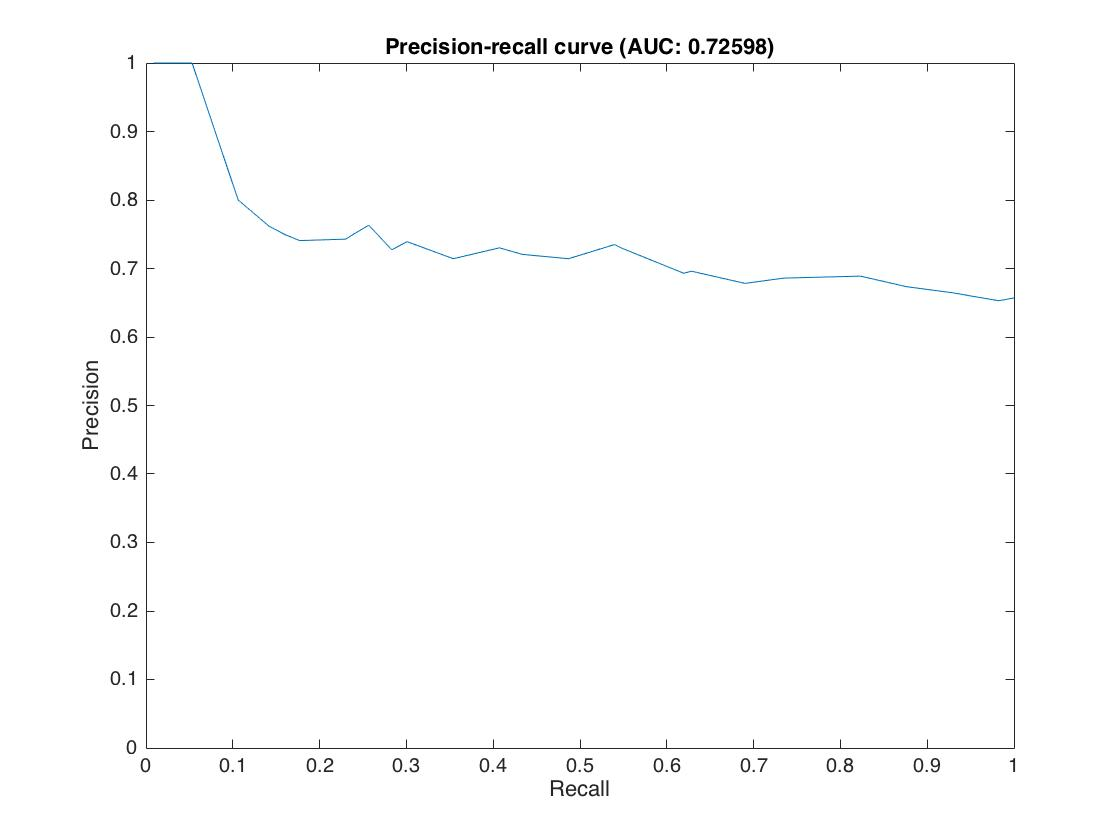
\includegraphics[width=\linewidth]{train_dso_test_dsi_prec_rec}
\endminipage
\caption{ROC curve and Precision-Recall curve for DSI-1 paired faces classification using trained data on DSO-1.}\label{fig:regiondetnormal}
\end{figure}

In the two previously considered cases, both of cross dataset classification, the differences between the two dataset compositions greatly influence the final evaluated performance. Almost all the images in the DSO-1, in fact, present similar lighting conditions. In addition, this dataset contains almost always the same people (and thus the same faces) in every picture. This fact makes the model trained using this dataset less expressive than the one trained using a more heterogeneous set of images, as in the case of DSI-1.

\subsubsection{Forgery detection performance}

In the following experiments, we used the proposed module to detect the face with the highest probability of being the fake face in an image tagged as fake by the classifier. 

In this round of experiments, we assume that the input image $I$ has already been classified as fake by the classifier (\emph{i.e.} at least one couple of faces has been classified as fake). 

We performed this kind of experiments using both DSO-1 and DSI-1 datasets. For each test in the suite it is reported:
\begin{itemize}
\item The training dataset (\textbf{Train})
\item The evaluation dataset (\textbf{Test})
\item The total number of faces detected in the images (\textbf{Faces})
\item The true positive rate (\textbf{TPR})
\item The classification accuracy (\textbf{ACC})
\item The classification precision (\textbf{PREC})
\item The classification recall (\textbf{REC})
\item The $F_1$ score (\textbf{F-Score})
\end{itemize}

Experimental results are collected in Table \ref{table:forgerydetections}.

\begin{table}[h!]
\centering
\begin{tabular}{l c c c c c c c} 
\hline \hline 
\textbf{N.} & \textbf{Train} & \textbf{Test} & \textbf{Faces} & \textbf{PREC} & \textbf{REC} & \textbf{ACC} & \textbf{F-Score} \\ [0.5ex]
\hline
1 & DSO-1 & DSO-1 &	540 & 0.58 & 0.89 & 0.81	& 0.64\\
2 & DSI-1 & DSI-1 &	133 & 0.56 & 0.95 & 0.75 & 0.66\\
3 &	DSO-1 & DSI-1 & 540 & 0.31 & 0.18 & 0.63 & 0.25\\ 
4 &	DSI-1 &	DSO-1 &	130 & 0.34 & 0.43 & 0.67 & 0.37\\[1ex]

\hline
\end{tabular}
\caption{Performance of face forgery detection module over single faces using non-uniform weights.}
\label{table:forgerydetections}
\end{table}


\section{Regions forgery detection module performance}

This section describes the experiments performed to evaluate the regional forgery detection module.

\subsection{Creating the training set}

Since the method is based on the classification of entire bands of images, in order to train the SVM classifiers were created two different training set with specific requirements:
\begin{itemize}
\item Each image must have only one spliced band (either horizontal or vertical)
\item The spliced region of the image must consist only int the whole band
\item The spliced region position in the image must be chosen randomly
\end{itemize}

Each image in the dataset must be shipped with its spliced band position as groundtruth (for performance evaluation).

For the two new training datasets, the DSO-1 and ColorChecker datasets were used respectively as source. Each generated dataset is splitted into two subset containing only vertical or horizontal spliced bands.

\begin{algorithm}[!h]
\begin{algorithmic}[1]
\State Let $d \in \{vertical, horizontal\}$ a direction
\State Let $S$ be the band size
\For {each image $i \in SourceDataset$}
\State Select another image $j$ randomly chosen from the same set with $i \neq j$
\State Resize $j$ to fit $i$
\State Select a band $b$ of direction $d$ randomly from $j$
\State Put $b$ in $i$ at the same original position
\State Save $i$ as image
\EndFor
\end{algorithmic}\caption{Spliced dataset creation algorithm}\label{alg:spliceddatasetcreation}
\end{algorithm}

The pseudocode used for generating the spliced datasets is proposed in Algorithm \ref{alg:spliceddatasetcreation}. That procedure is repeated for both DSO-1 and ColorChecher as $SourceDataset$ and for each direction. We called \emph{SplicedDSO} the dataset generated from DSO-1, \emph{SplicedCC} the one from ColorChecker. Both have 200 images vertically and horizontally spliced.

\begin{figure}[!htb]
\minipage{0.48\textwidth}
  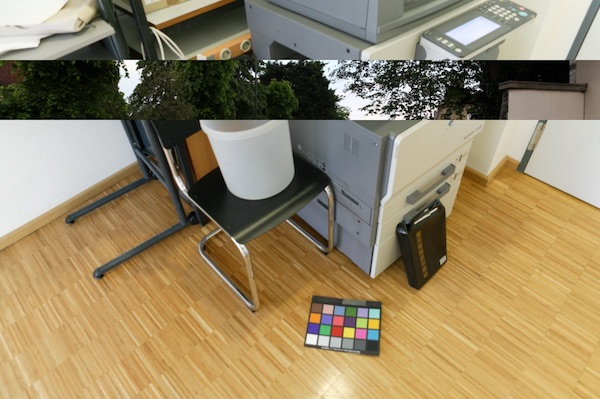
\includegraphics[width=\linewidth]{splicedcchor}
\endminipage\hfill
\minipage{0.48\textwidth}
  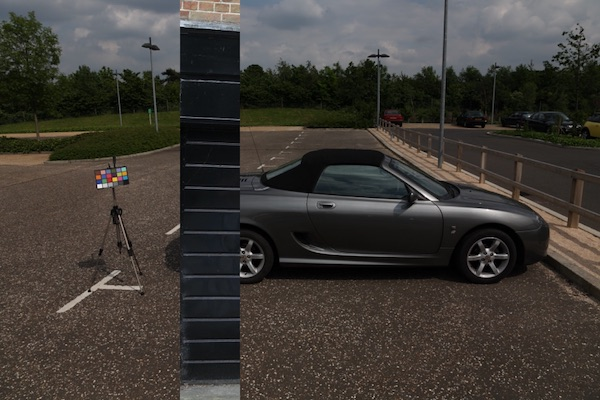
\includegraphics[width=\linewidth]{splicedccver}
\endminipage
\caption{Example images from the generated \emph{SplicedCC} dataset. Left with horizontal spliced band, right with vertical.}\label{fig:splicedccsamples}
\end{figure}

\begin{figure}[!htb]
\minipage{0.48\textwidth}
  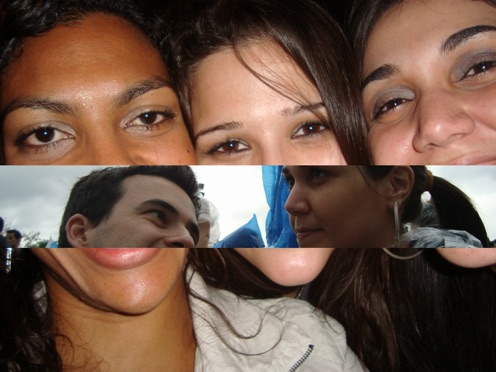
\includegraphics[width=\linewidth]{spliceddsohor}
\endminipage\hfill
\minipage{0.48\textwidth}
  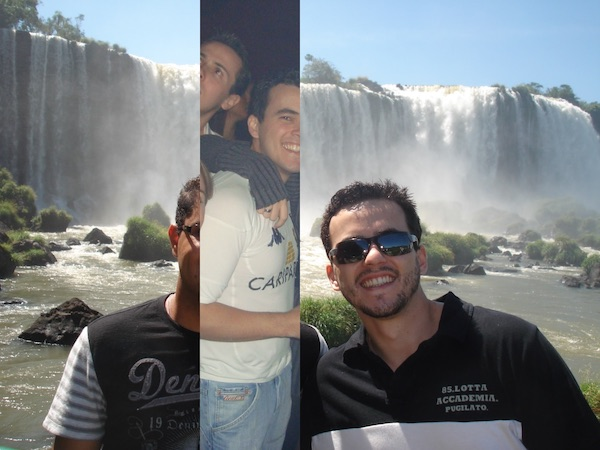
\includegraphics[width=\linewidth]{spliceddsover}
\endminipage
\caption{Example images from the generated \emph{SplicedDSO} dataset. Left with horizontal spliced band, right with vertical.}\label{fig:spliceddsosamples}
\end{figure}

Figures \ref{fig:splicedccsamples} and \ref{fig:spliceddsosamples} show two examples of generated images from both dataset. 

\subsection{Evaluating module performance}

The proposed method output consists in a\emph{ detection map} related to the analyzed image. In order to evaluate the performance of the module, we consider the single pixel classification accuracies. The evaluation dataset for all the experiments is the original DSO-1 dataset (considering only the spliced images).

Given a set of $m$ images as validation test, for each test in the suite:
\begin{enumerate}
\item Let $I$ the $i$-th analyzed image, a detection map $D_i$ is computed with our module.
\item Let $\mathcal{P}_i$ the subset of pixels in the image corresponding to the spliced region and let $\mathcal{S}_{\mathcal{P}_i}$ their corresponding values extracted from $D$. Finally, let $N_i$ the subset of pixels in the image corresponding to its original part and let $\mathcal{S}_{\mathcal{N}_i}$ their corresponding values extracted from $D_i$.
\item Step 1 and 2 are repeated for each image in the validation step, joining the resulting sets of scores:
$$
\mathcal{S}_{\mathcal{P}} = \cup_{i = 1}^{m} \mathcal{S}_{\mathcal{P}_i}
$$
$$
\mathcal{S}_{\mathcal{N}} = \cup_{i = 1}^{m} \mathcal{S}_{\mathcal{N}_i}
$$
\end{enumerate}

The two resulting sets of scores, $\mathcal{S}_{\mathcal{P}}$ and $\mathcal{S}_{\mathcal{N}}$ are used for evaluating overall performances.

The size of the evaluation dataset is limited to 25 image due the  required computational time. In the classification stage, we used an SVM classifier with an RBF kernel, and classical grid search for adjusting parameters in training samples \cite{bishop2007pattern}.

Experimental results are collected in Table \ref{table:performanceregionaldet}.

\begin{table}[h!]
\centering
\begin{tabular}{l c c c c c} 
\hline \hline 
\textbf{Test case} & \textbf{Train} & \textbf{RC} & \textbf{ACC} & \textbf{AUC} &\textbf{ F-Score} \\ [0.5ex]
\hline
Test 1 & - & Median & 0.49 & 0.32 & 0.25\\
Test 2 & - & Global & 0.52 & 0.40 & 0.27\\
Test 3 & SplicedCC & Median & 0.54 & 0.53 & 0.26\\
Test 4 & SplicedCC & Global & 0.57 & 0.57 & 0.31\\
Test 5 &	 SplicedDSO & Median & 0.53 & 0.50 & 0.27\\
Test 6 &	 SplicedDSO & Global & 0.61 & 0.63 & 0.33\\ [1ex]
\hline
\end{tabular}
\caption{Performance of region forgery detection module.}
\label{table:performanceregionaldet}
\end{table}

\subsection{Test cases}

\subsubsection{Performance without training}

\begin{figure}[!htb]
\minipage{0.42\textwidth}
  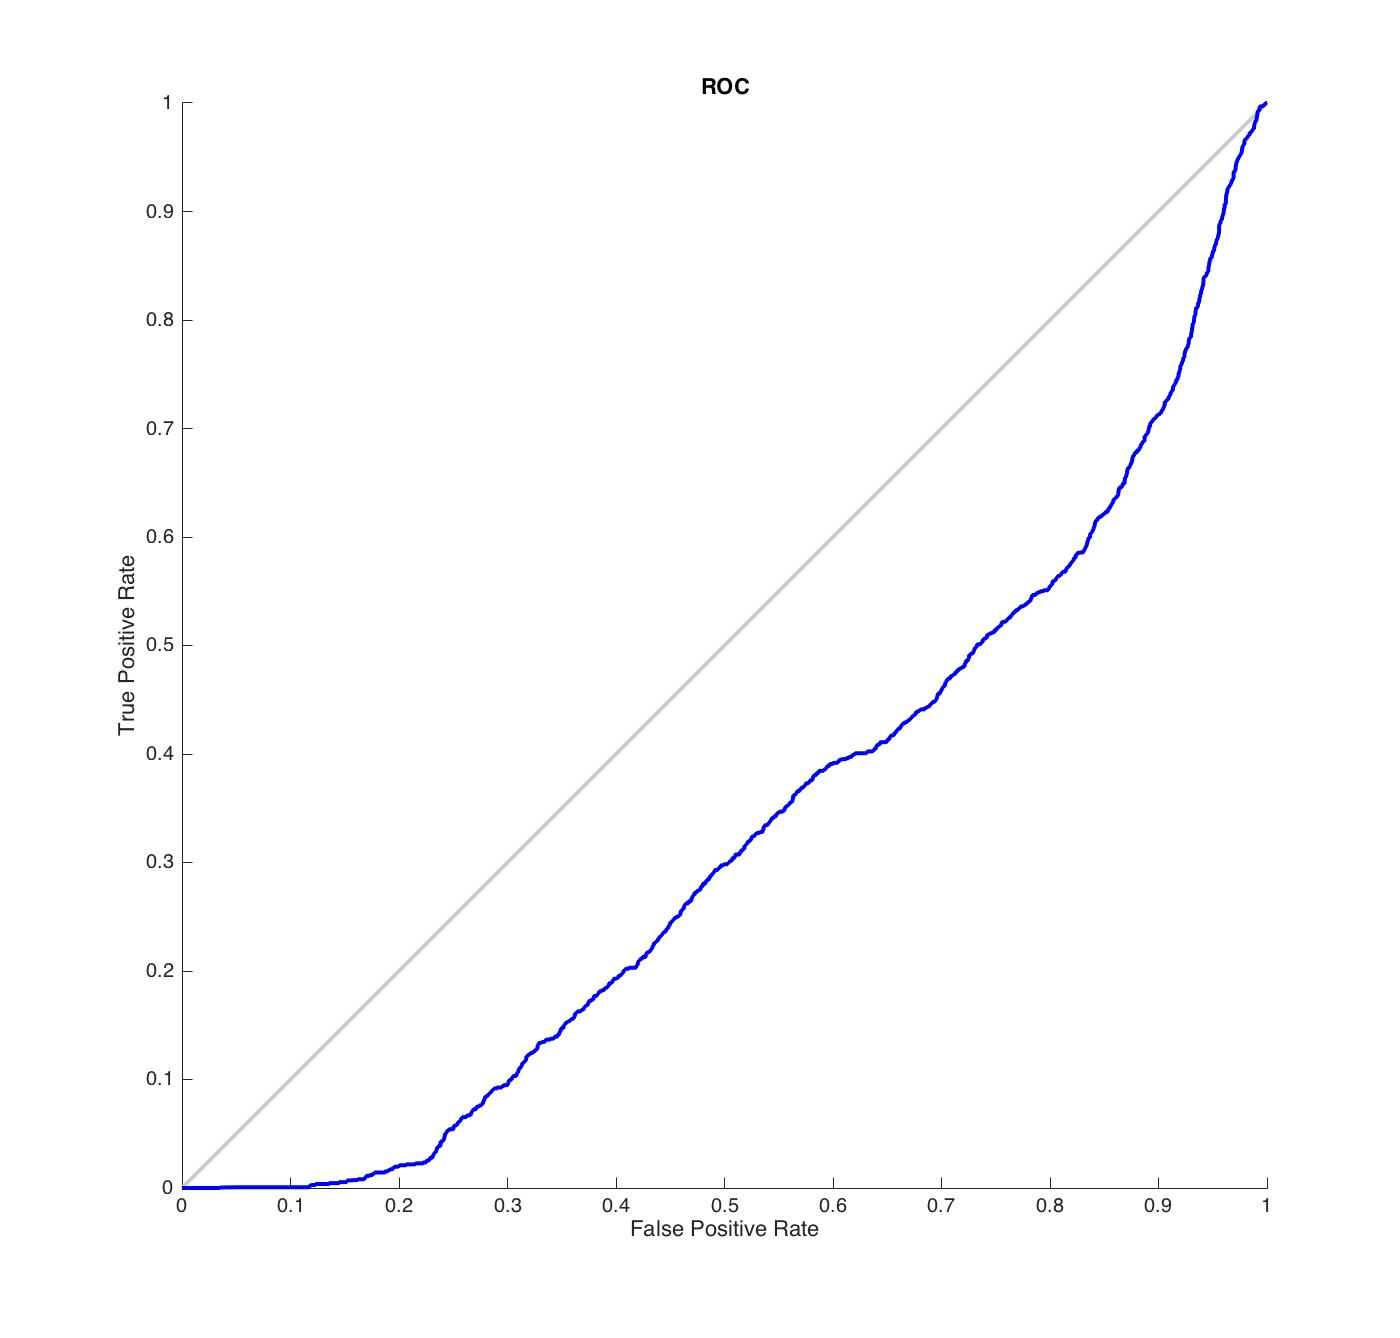
\includegraphics[width=\linewidth]{train_cc/roc_normal}
\endminipage\hfill
\minipage{0.53\textwidth}
  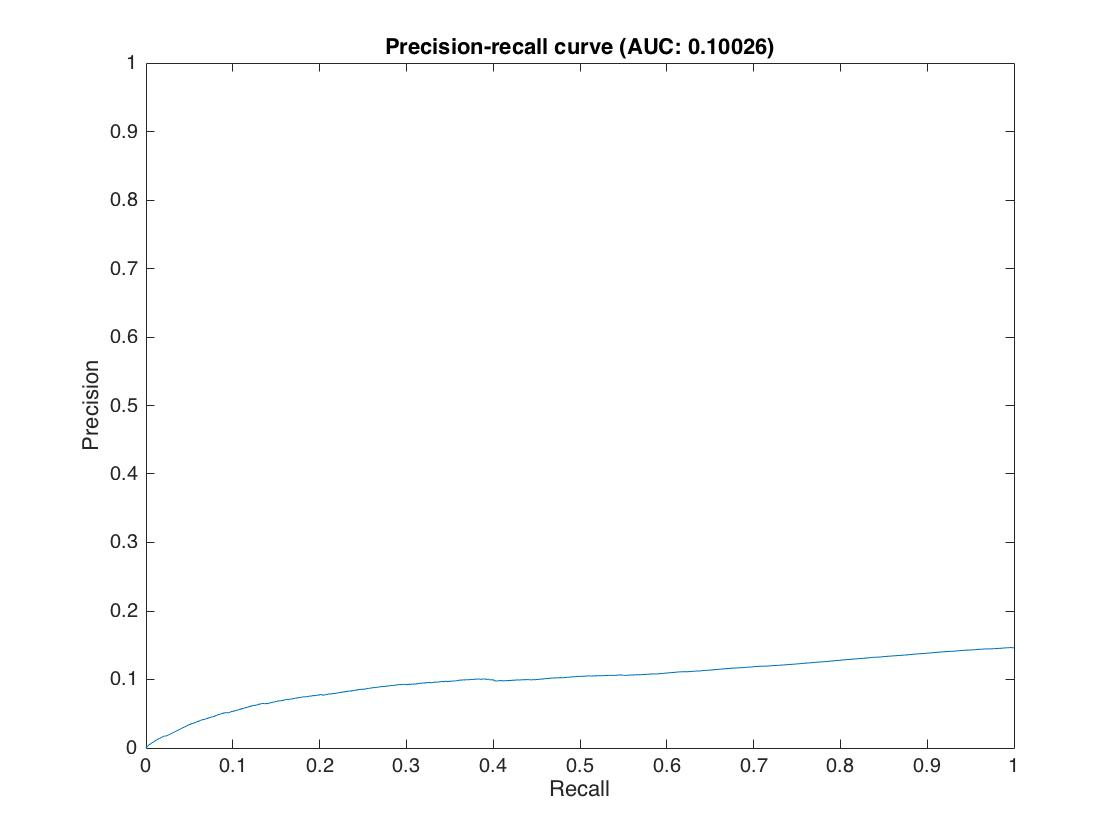
\includegraphics[width=\linewidth]{train_cc/prec_rec_normal}
\endminipage
\caption{ROC curve and Precision-Recall curve for classification without training, using the median reference value.}\label{fig:regiondetnormal}
\end{figure}

\begin{figure}[!htb]
\minipage{0.42\textwidth}
  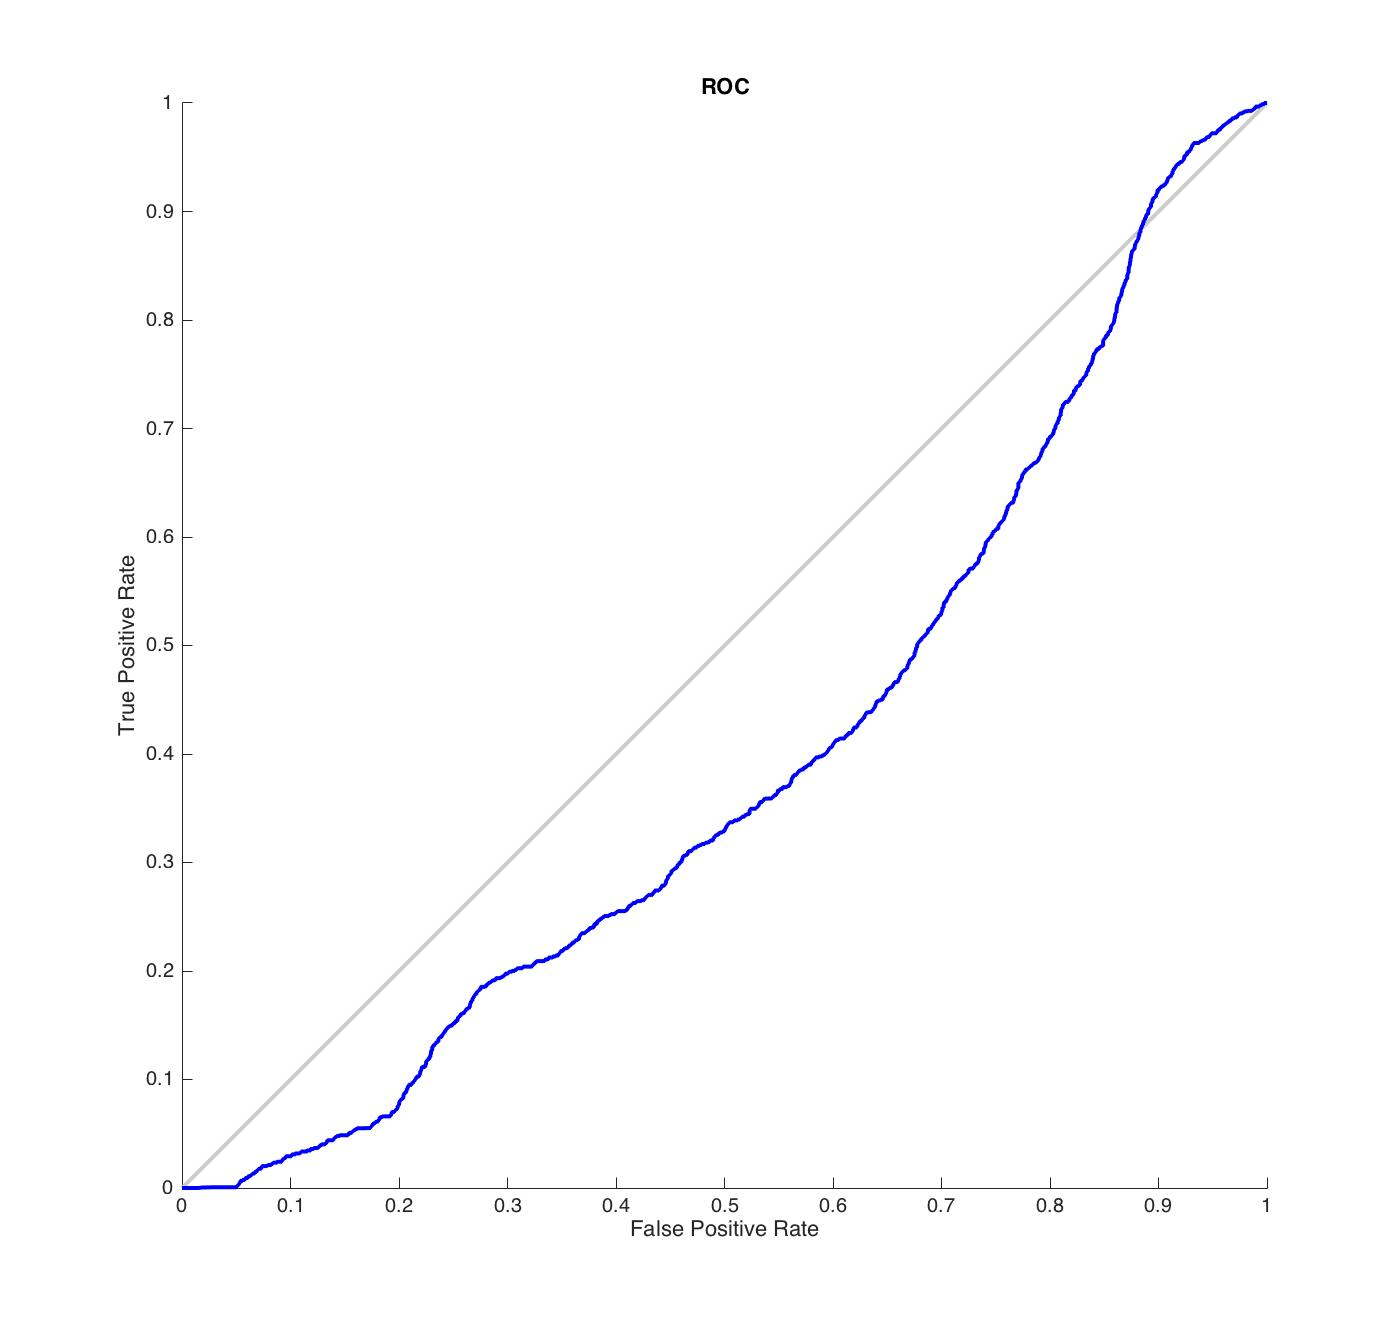
\includegraphics[width=\linewidth]{train_cc/roc_normal_global}
\endminipage\hfill
\minipage{0.53\textwidth}
  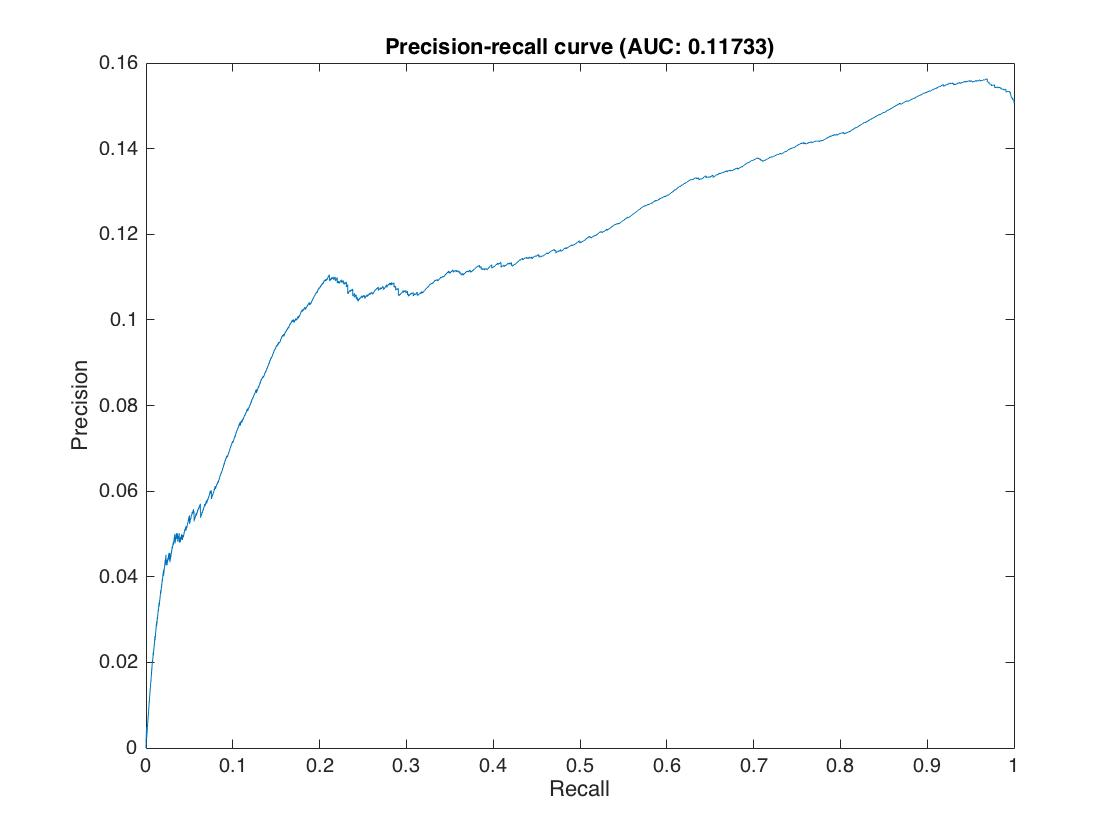
\includegraphics[width=\linewidth]{train_cc/prec_rec_normal_global}
\endminipage
\caption{ROC curve and Precision-Recall curve for classification without training, using the global reference value.}\label{fig:regiondetnormal}
\end{figure}

\subsubsection{Performance with SVM training over \emph{SplicedCC}}

\begin{figure}[!htb]
\minipage{0.42\textwidth}
  \includegraphics[width=\linewidth]{train_cc/roc_svm}
\endminipage\hfill
\minipage{0.53\textwidth}
  \includegraphics[width=\linewidth]{train_cc/prec_rec_svm}
\endminipage
\caption{ROC curve and Precision-Recall curve for classification with SVM training on \emph{SplicedCC}, using the global reference value.}\label{fig:regiondetnormal}
\end{figure}

\begin{figure}[!htb]
\minipage{0.42\textwidth}
  \includegraphics[width=\linewidth]{train_cc/roc_svm_global}
\endminipage\hfill
\minipage{0.53\textwidth}
  \includegraphics[width=\linewidth]{train_cc/prec_rec_svm_global}
\endminipage
\caption{ROC curve and Precision-Recall curve for classification with SVM training on \emph{SplicedCC}, using the global reference value.}\label{fig:regiondetnormal}
\end{figure}

\subsubsection{Performance with SVM training over \emph{SplicedDSO}}

\begin{figure}[!htb]
\minipage{0.42\textwidth}
  \includegraphics[width=\linewidth]{train_dso/roc_svm}
\endminipage\hfill
\minipage{0.53\textwidth}
  \includegraphics[width=\linewidth]{train_dso/prec_rec_svm}
\endminipage
\caption{ROC curve and Precision-Recall curve for classification with SVM training on \emph{SplicedDSO}, using the global reference value.}\label{fig:regiondetnormal}
\end{figure}

\begin{figure}[!htb]
\minipage{0.42\textwidth}
  \includegraphics[width=\linewidth]{train_dso/roc_svm_global}
\endminipage\hfill
\minipage{0.53\textwidth}
  \includegraphics[width=\linewidth]{train_dso/prec_rec_svm_global}
\endminipage
\caption{ROC curve and Precision-Recall curve for classification with SVM training on \emph{SplicedDSO}, using the global reference value.}\label{fig:regiondetnormal}
\end{figure}

